\section{Zielsetzung}
	
	Die Vakuumtechnik befasst sich mit der Erzeugung, Aufrechterhaltung und Messung eines Vakuums.
	Diese Technik ist wichtig für die Industrie und Forschung um reine Produkte herzustellen und ungestörte Messungen durchzuführen.
	Moderne Versuche erreichen Drücke, bis zu etwas unter $\SI{10e-11}{\milli\bar}$.
	In diesem Versuch werden allgemeine theoretische Begriffe in Verbindung mit Vakua erläutert.
	Experimentiell wird das Saugvermögen einer Drehschieberpumpe und einer Turbomolekularpumpe bestimmt.
	Dazu werden jeweils einige Evakurierungskurven aufgenommen und Leckratenmessungen durchgeführt.
	

\section{Theorie}
	
	\subsection{Vakuum}
		
		Allgemein wird von einem Vakuum gesprochen, sobald der Druck innerhalb eines Gefäßes niedriger als sein Umgebungsdruck ist.
		Da der niedrigste auf der Erde vorkommende Atmosphärendruck in großer Höhe bei $p = \SI{300}{\milli\bar}$ liegt, wird ab dann von einem Vakuum gesprochen.
		Es ist in diesem Versuch eine gute Näherung wenn wir bei dem vorliegendem Gas von idealem Gas sprechen. 
		Dies bedeutet, dass jegliche Wechselwirkungen zwischen Teilchen nur durch vollkommen elastische Stöße passieren und die Gasteilchen keine Ausdehnung besitzen.
		Wenn dies angenommen wird, kann das Gas auch mit der Idealen Gasgleichung
		\begin{equation}
			p \cdot V = N \cdot \symup k _{\symup b} \cdot T
		\end{equation}
		beschrieben werden.
		Hier ist $p$ der Druck, $V$ das Volumen, $N$ die Teilchenzahl, $\symup k _{\symup B}$ die Boltzmann Konstante und $T$ die Temperatur. 
		Ein Spezialfall dieser Gleichung ist das Gesetz von Boyle-Mariotte. Dieses besagt, dass bei konstanter Temperatur
		\begin{equation}
			p \propto V^{-1}
		\end{equation}
		ist.
		Der Druck ist als Kraft pro Fläche definiert, es gilt:
		\begin{equation}
		\SI{1}{\pascal} = \SI{0.01}{\milli\bar} = \SI{1}{\newton\per\metre\squared}.
		\end{equation}

	\subsection{Fachbegriffe}
	
		\begin{itemize}
			\item
			Die mittlere freie Weglänge beschreibt die durschnittliche Fluglänge eines Gasteilchens zwischen zwei Kollisonen mit anderen Gasteilchen.
			Diese ist relevant für das Verhalten unterschiedliche Verhalten und die Funktionsweise unterschiedlicher Vakuumpumpen.\\
			(Quelle: \cite{wiki:mfg})

			\item
			Die Sorption bezeichnet den Vorgang einer Anreicherung eines Stoffes. 
			Hier beschreibt die Absorption, wenn der Stoff innerhalb einer Phase aufgenommen wird. 
			Ein Beispiel ist die Aufnahme von Neutronen in den Atomkernen eines Festkörpers.
			Adsorption ist im Gegensatz zur Absortion die Anlagerung auf der Oberfläche oder Grenzfläche eines Stoffes.
			Die Desorption beschreibt gegensätzlich einen Prozess bei dem Atome oder Moleküle die Oberfläche eines Festkörpers verlassen und in die Gasphase übergehen.\\
			(Quelle: \cite{wiki:sorp})
			
			\item
			Lecks beschreiben Prozesse die das Vakuum reduzieren. Es wird dabei zwischen realen und virtuellen Lecks unterschieden.
			Reale Lecks sind Prozesse die von außerhalb der Vakuumanlage messbar sind. Eine nicht korrekt verschlossene Verbindung ist zum Beispiel ein reales Leck.
			Virtuelle Lecks entstehen zum Beipiel durch Einschlüsse in der Vakuumanlage, welche sich mit zunehmendem Druck freisetzten.
			Diese Art von Lecks sind von außen nicht zu messen und müssen beim Aufbau oder in der Produktion der Vakuumkomponenten verhindert werden.
			Einzelne Gaseinschlüsse können zum Beispiel bei der Produktion durch Ultraschall zu größeren Gasblasen diffundiert werden, welche dann an die Oberfläche steigen und austreten.
			In diesem Versuch sind Lecks und Desorption mitunter dafür verantwortlich, dass nur gewisse Vakuumbereiche erreicht werden können. \\
			(Quelle: \cite{pfeiffer:grund})

			\item
			Im Allgemeinen beschreibt das Saugvermögen $S$ einer Vakuumpumpe, wie viel Gas sie aus dem Rezipienten pumpen kann. 
			Also die zeitliche änderung von Volumen oder Druck.
			\begin{equation}
				S = \frac{\text{d}V}{\text{d}t} = - \frac{V}{p} \frac{\text{d}p}{\text{d}t}
			\end{equation}
			Um dieses zu Bestimmen werden in diesem Versuch Evakuierungskurven, also Druckänderungen als Funktion der Zeit aufgenommen.
		\end{itemize}

	\subsection{Vakuumbereiche}

		\noindent
		Physikalisch sind mehrere Vakuumbereiche definiert, da mit abnehmendem Druck die Teilchendichte in einem Volumen reduziert wird.
		Mit abnehmender Teilchenzahldichte steigt die mittlere freie Weglänge. 
		Die Anzahl an Stöße unter den Gasteilchen nimmt ab.
		Weiterhin lässt sich aus der idealen Gasgleichung $p \cdot V = n \cdot k_\t{B} \cdot T $, auch wenn die Teilchenzahl nicht konstant ist, doch ablesen, dass die Temperatur mit abnehmendem Druck fällt. 	
		Mit abnehmender Temperatur sinkt nach der Maxwell-Boltzmann Verteilung auch die Teilchengeschwindigkeit.	
		Diese bestimmt zum Beispiel wie ein Gas durch einen Leiter strömt.
		
		\begin{itemize}
			\item
			Im ersten relevanten Druckbereich wird von einem Grobvakuum gesprochen. Dieses ist zwischen $\SI{300}{\milli\bar}$ und $\SI{1}{\milli\bar}$ definiert.
			In diesem Bereich findet allgemein viskose Strömung statt, in der der Großteil der Stöße zwischen den Gasteilchen untereinander und nicht mit der Gefäßwand stattfinden.
			Es wird abhängig von der Teilchengeschwindigkeit, der Teilchendichte und der Gefäßgröße zwischen laminarer und turbulenter Strömung unterschieden. 

			\item
			Das Feinvakuum ist zwischen $\SI{1}{\milli\bar}$ und $\SI{e-3}{\milli\bar}$ definiert. Hier findet Knudsen-Strömung statt.
			Knudenströmung beschreibt Strömung bei der der Leitungsdurchmesser vergleichbar mit der mittleren freien Weglänge ist.
			Hier wechselwirken die Gasteilchen hauptsächlich mit den Wänden des Gefäßes.

			\item
			Es wird ab einem Druck von $\SI{e-3}{\milli\bar}$ bis $\SI{e-8}{\milli\bar}$ von Hochvakuum gesprochen. Von Ultrahochvakuum ist ab $\SI{e-8}{\milli\bar}$ die Rede.	
			In diesen beiden Druckbereichen findet nur noch molekulare-Strömung statt.
			Dies bedeutet, dass die Teilchen untereinander fast nicht mehr Wechselwirken. 
			Hier ist die mittlere freie Weglänge größer als die Weite des Strömungskanals.
		\end{itemize}
		Diese unterschiedlichen Strömungsarten haben hohe Relevanz bei praktischen Anwendungen, da zum Beispiel das effektive Saugvermögen von Vakuumpumpen beeinträchtigt werden kann.
		\begin{figure}
			\centering
			\includegraphics[width=0.4\linewidth]{"latex/images/Strömungen.PNG"}
			\caption{Ein schematische Darstellung des Strömungsverhalten bei unteschiedlichen mittleren freien Weglängen.
				 Hier stellen blaue Pfeile, Teilchen mit geringer und grüne Pfeile, Teilchen mit langer mittleren freien Weglänge dar. \protect Quelle: \cite{pfeiffer:pump}}
			\label{fig:stroe}
		\end{figure}  
		Wie in Abbildung \ref{fig:stroe} schematisch dargestellt ist, führen große mittlere freie Weglängen und kleine Leiterdurchmesser zu chaotischem Flussverhalten der Teilchen.
		Im Grobvakuum reichen kleinere Leitungsdurchmesser, damit laminare Stömung sicher gestellt ist.
		Im Ultrahochvakuum sollten größere Leitungsdurchmesser benutzt werden um hohe Flussraten sicherzustellen.\\
		(Quelle: \cite{pfeiffer:grund})

	\subsection{Arten der Vakuumerzeugung}	
		
		\noindent
		Vakuumpumpen können sich stark in ihrer Funktionsweise abhängig vom Arbeitsbereich unterscheiden.
		Der größte Unterschied liegt zwischen gasbindenden und gasfördenden Vakuumpumpen, wobei sich gasfördernde Pumpen noch einmal in verdrängende und kinetische Pumpen unterteilen.
		\begin{itemize}
		\item
		Gasbindende Vakuumpumpen funktionieren durch Sorption, indem Gasteilchen zum Beispiel mittels Physisorption gebunden werden. 
		Dieses Prinzip ergibt erst bei bereits sehr gutem Vakuum Sinn. 
		Bei hohem Druck, ist die Teilchendichte noch sehr hoch und die Pumpe kann nur einen kleinen Teil der noch vorhandenen Teilchen in der Gasphase aufnehmen.
		Ist das Vakuum jedoch sehr hoch, kann die gasbindende Vakuumpumpe einen großen Teil der noch vorhandenen Teilchen aufnehmen und somit das Vakuum weiter verbessern oder aufrecht erhalten.
		\item
		Gasfördernde Vakuumpumpen fördern Gas durch abgeschlossene Volumina, welche komprimiert werden oder sich ausdehnen.
		Hier wird das Gesetzt von Boyle-Mariotte ausgenutzt, dass bei konstanter Temperatur, das Volumen antiproportional zum Druck ist.
		Beim Ausgleichen der Drücke fließen dann Teilchen aus dem Rezipienten in die Pumpkammern oder aus den Pumpkammern in die Umgebung. 
		\item
		Kinetische Pumpen erhöhen das Vakuum, indem Gasteilchen in Richtung der Pumprichtung beschleunigt werden.
		Auch dieses Vakuumerzeugungsprinzip hat bei Atmosphärendruck einige Probleme und benötigt ein Vorvakuum.
		Ist nicht bereits ein Vorvakuum vorhanden, so kann aufgrund der hohen Teilchendichte, der Widerstand durch die vielen einzelnen Kollisionen mit den Vakuumkomponenten zu hoch sein.
		Zum einen werden also die Leistungsanforderungen und der Verschleiß der Vakauumpumpe durch ein Vorvakuum reduziert.
		Weiterhin funktioniert ab einem gewissen Druck, die Funktionsweise der Vakuupumpe nicht mehr.
		Die mittlere freie Weglänge ist dann nicht mehr weit genug und die beschleunigten Teilchen verlieren ihre Bewegungsrichtung zu früh durch Stöße mit anderen Gasteilchen.
		\end{itemize}
		\subsubsection{Drehschiebervakuumpumpe} 
						
			\begin{figure}
				\centering
				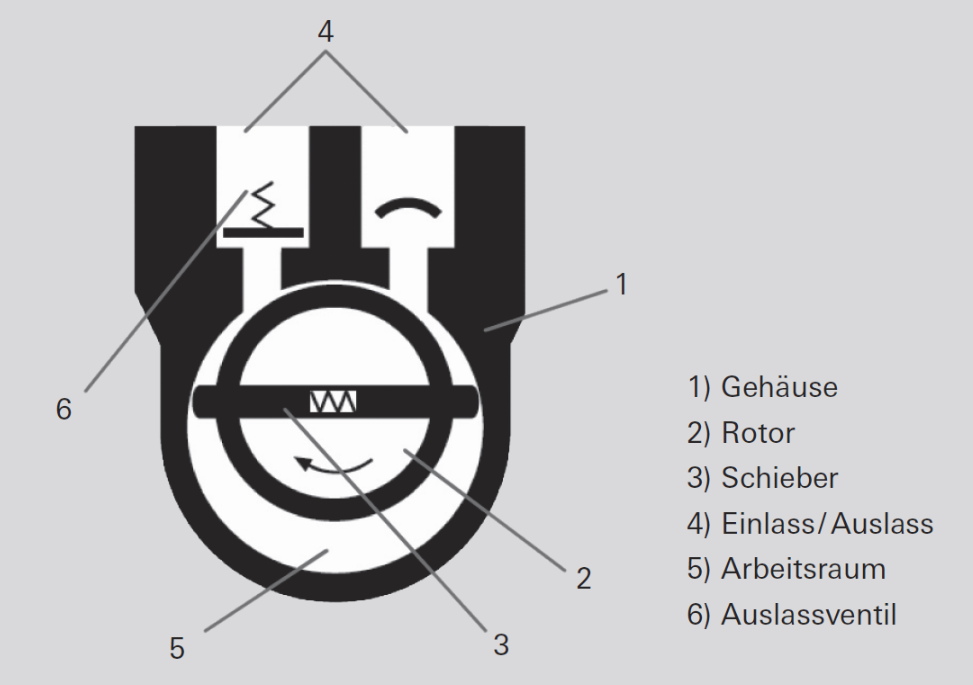
\includegraphics[width=0.5\linewidth]{"latex/images/Drehschieber.png"}
				\caption{Der schematische Aufbau einer Drehschiebervakuumpumpe. \protect Quelle: \cite{pfeiffer:pump}}
				\label{fig:dreh}
			\end{figure}  

			\noindent
			Die Drehschieberpumpe ist eine Rotationsverdrängerpumpe und somit aus der Klasse der Gasfördernden Vakuumpumpen.
			Sie besteht aus dem Gehäuse (1), dem eingebauten Rotor(2), den mit Flieh- und Federkraft radial bewegten Schiebern(3) und dem Ein- bzw. Auslass(4).
			Das Innere des Arbeitsraumes(5) wird durch den Stator, den Rotor und die Schieber in mehrere Bereiche eingeteilt. 
			Wie bereits beschrieben, entsteht durch Expansion und Kompression der Volumina in den Arbeitsbereiche, ein Teilchenstrom vom Einlass zum Auslass. 
			Eine zweistufige Drehschieberpumpe kann Drücke bis zu $\SI{5e-4}{\milli\bar}$ erreichen. 
			In diesem Versuch wird jedoch nur eine einstufige Pumpe mit einem Enddruck von $p = \SI{2.1 e-2}{\milli\bar}$ genutzt.
			Ein Nachteil der Drehschieberpumpe ist, dass unter anderem zum Abschließen der Kammern, Öl verwendet wird.
			Mittels Desorption können daher Moleküle aus dem Öl in den Rezipienten übergehen und dessen Vakuum verunreinigen.	 

		\subsubsection{Turbomolekularpumpe}
		
			\noindent
			Turbomolekularpumpen sind turbinenähnliche kinetische Vakuumpumpen.\\ 
			In ihrem Gehäuse ist ein mehrstufiger Rotor mit Schaufeln.
			Zwischen den Rotorscheiben sind beschaufelte Statorscheiben mit spiegelverkehrter Symmetrie zu den Rotorscheiben.
			Die Rotorscheiben drehen sich je nach größe der Pumpe mit bis zu einigen kHz, in diesem Versuch mit bis zu $\SI{1350}{\hertz}$.
			Das Ziel ist, dass die Schaufeln eine Rotationsgeschwindigkeit ähnlich der mittleren Teilchengeschwindigkeit haben.
			Durch Wechselwirkung mit den Rotor und Statorschaufeln werden die Gasteilchen in Pumprichtung beschleunigt.
			Eine Voraussetzung für diese Funktionsweise ist, dass in der Pumpe Molekulare-Strömung vorliegt, die Teilchen also fast nicht mehr untereinander wechselwirken.
			Die mittlere freie Weglänge muss größer sein, als die Abstände zwischen Rotor und Statorscheiben, damit die Teilchen ihre Bewegungsrichtung bei behalten.\\
			(Quelle: \cite{pfeiffer:pump})
			  					
		\subsubsection{Messung der p(t)-Kurve}
			
			\noindent
			Wird von einem idealem Gas ausgegangen und die Gleichung:
			\begin{equation}
				p \cdot V = \text{const}
			\end{equation}
			nach der Zeit abgeleitet, entstehen auf der linken Seite zwei Summanden. \\
			Wird mit dem Druck $p$ multipliziert kann die zeitliche Ableitung des Volumens als das Saugvermögen $S$ identifiziert werden.\\
			Durch Verschieben der Terme entsteht folgende Gleichung:
			\begin{equation}
				\frac{\text{d}V}{\text{d}t} = S = - \frac{V}{p} \frac{\text{d}p}{\text{d}t}
			\end{equation}
			Diese Differentialgleichung wird mittels einer Exponentialfunktion mit dem Saugvermögen $S$, dem konstantem Rezipienten Volumen $V_0$, dem Anfangsdruck $p_0$ und der Zeit $t$ im Exponenten gelöst:
			\begin{equation}
				p(t) = p_0 \text{exp}\left( - \frac{S}{V_0}t \right)
			\end{equation}
			Jedoch muss beachtet werden, dass alle Vakuumpumpen einen gewissen Enddruck $p_\text{E}$ haben. 
			Sobald dieser Druck erreicht ist, kann die Pumpe den Druck nicht weiter erhöhen und es entsteht ein Gleichgewicht zwischen Saugvermögen und 
			vakuumreduzierenden Prozessen wie Desorption oder Lecks.\\
			Der Gleichgewichtsdruck wird in der Evakuierungskurve durch Verschieben und Skalieren der Exponentialfunktion eingerechnet:
			\begin{equation}
				p(t) = (p_0 - p_\text{E}) \text{exp}\left( - \frac{S}{V_0}t \right) + p_\text{E}
				\label{eqn:druckkurve}
			\end{equation}
			Mit dieser Formel lässt sich aus der Evakuierungskurve eine Schätzung für das Saugvermögen einer Vakuumpumpe berechnen.
			Jedoch muss beim Auswerten darauf geachtet werden, dass Vakuumpumpen zum Beispiel in unterschiedlichen Strömungsarten, auch verschiedene Saugvermögen aufweisen.
			
		\subsubsection{Leckratenmessung}
			
			\noindent
			Zur Berechnung des Saugvermögens mittels Leckratenmessung muss zunächst die Leckrate $Q$ mittels des Gleichgewichtsdruck $p_\text{g}$ definiert werden:
			\begin{equation}
				S = \frac{Q}{p_\text{g}},
			\end{equation}
			und
			\begin{equation}
				Q = V_0 \frac{\Delta p}{\Delta t}.
			\end{equation}
			Hieraus folgt ein Ausdruck für das Saugvermögen der Vakuumpumpe:
			\begin{equation}
				S = \frac{V_0}{p_\text{g}} \cdot \frac{\Delta p}{\Delta t.}
			\end{equation}
			Aus der Steigung $\frac{\text{d}p}{\text{d}t}$ lässt sich bei unterschiedlich eingestellten Gleichgewichtsdrücken $p_\text{g}$, das Saugvermögen mit Hilfe der Leckratenmessung bestimmen.
		\subsubsection{Leitwert}

			\noindent
			Bei all diesen Berechnungen ist zu bedenken, dass das theoretische Saugvermögen $S_0$ immer durch die Vakuumanlage reduziert wird.
			Dieser Effekt wird durch den Leitwert $L$ des Rezipienten beschrieben. 
 			Er gibt den reziproken Strömungswiderstand der Schläuche und Verbindungen an.
			Das effektive Saugvermögen $S_\text{eff}$, dass tatsächlich am Rezipienten ankommt, berechnet sich damit zu:
			\begin{equation}
				S_\text{eff} = \frac{S_0 \cdot L}{S_0 + L}.
			\end{equation}

	\subsection{Arten der Vakuummessung}
		
		\subsubsection{Pirani-Vakuummeter}
			
			\noindent
			Das Pirani-Vakuummeter arbeitet optimal im Bereich des Feinvakuums.
			Es nutzt aus, dass in diesem Druckbereich die Wärmeleitfähigkeit proportional zum Druck ist. 
			Der Wärmetransport geschieht hier primär durch direkte Stöße von Gasteilchen untereinander. 
			Die Messung erfolgt über einen Draht in dem Rezipienten, durch den ein konstanter Strom fließt.
			Nun kann mittels einer Wheatstone-Brücke der Widerstand dieses Leiters und somit die Temperatur des Drahtes bestimmt werden.
			Da der Draht sich abhängig von dem Druck im Rezipienten unterschiedlich schnell abkühlt, kann mit dieser Methode auch der Druck in dem Rezipienten bestimmt werden.

		\subsubsection{Penning-Vakuummeter}

			\noindent
			Das Penning-Vakuummeter ist ein Kalt-Ionisations-Vakuumeter.\\
			Es arbeitet im Hoch- und Ultrahochvakuum. 
			Es beruht darauf, dass mittels elektrischer Feldemission ein elektrisches Feld Elektronen freigesetzt werden.
			Die frei werdenden Elektronen werden zur Anode beschleunigt und ionisieren auf ihrem Beschleunigungsweg weitere Gasatome.\\
			Diese Ionen werden dann zu der Kathode beschleunigt und erzeugen dort einen Ionenstrom, welcher ein Maß für das Vakuum ist.

		\subsubsection{Bayard-Alpert-Vakuummeter}

			\noindent
			Das Bayard-Alpert-Vakuummeter ist eine Heiß-Ionisations-Vakuumeter.\\ 
			Es arbeitet sehr analog zu dem Penning-Vakuumeter.
			Der einzige Unterschied ist, dass die Elektronen durch thermische Emission freigesetzt werden.
		
		\subsubsection{Piezo-Vakuummeter}
			
			\noindent
			Ein Piezo-Vakuumeter vermisst das Vakuum direkt, indem es die Kraft des Gases auf eine Oberfläche misst. 
			Da mit immer besser werdendem Vakuum auch die Kraft abnimmt, eignet sich dieses Vakuummeter am besten bis zum Grobvakuum ($\SI{1000}{\milli\bar}$ bis $\SI{1}{\milli\bar}$).
			Die konkrete Messung erfolgt mittels Piezo-Kristallen, welche bei Kompression eine elektrische Spannung erzeugen, die dann abgelesen wird.
			Aufgrund der ähnlichen Arbeitsbereiche werden, wie auch in diesem Versuch, Piezo- und Pirani-Vakuummeter oft in einem Messgerät kombiniert.

			\newpage
